\documentclass{VUMIFPSkursinis}
\usepackage{algorithmicx}
\usepackage{algorithm}
\usepackage{algpseudocode}
\usepackage{amsfonts}
\usepackage{amsmath}
\usepackage{bm}
\usepackage[margin=50pt]{caption}
\usepackage{color}
\usepackage{float}
\usepackage{graphicx}
\usepackage{listings}
\usepackage{subfig}
\usepackage{wrapfig}
\usepackage{fontspec}
\usepackage{todonotes}
\usepackage{pdfpages}
\usepackage{tlatex}
\usepackage{multicol}
\usepackage{changepage}   % for the adjustwidth environment
%\newcommand{\TD}[1]{\todo[inline, color=red!40]{#1}}

% Titulinio aprašas
\university{Vilniaus universitetas}
\faculty{Matematikos ir informatikos fakultetas}
\department{Programų sistemų bakalauro studijų programa}
\papertype{Kursinis darbas}
\title{Raft Algoritmo Ra Praplėtimų Tyrimas}
\titleineng{Investigation of Raft Algorithm Ra Extensions}
\status{3 kurso 1 grupės studentas}
\author{Edvardas Dlugauskas}
% \secondauthor{Vardonis Pavardonis}   % Pridėti antrą autorių
\supervisor{dr. Karolis Petrauskas}
\date{Vilnius – \the\year}

% Nustatymai
\definecolor{back}{RGB}{245, 245, 245}    % nauja spalva (pilka, tinkanti kodo fonui)
\lstdefinestyle{fancycode}{                        
% aplinkos lstlisting nustatymai graziam kodo iterpimui:
% KODE REIKES NURODYTI \begin{lstlisting}[style=fancycode]
    backgroundcolor = \color{back},           % colour for the background
    commentstyle = \it\color{magenta},        % style of comments
    keywordstyle = \color{blue},              % style of keywords
    numberstyle = \tiny\color{black},         % style used for line-numbers
    stringstyle = \color{ForestGreen},        % style of strings
    basicstyle = \linespread{1}\footnotesize, % font size/family/etc. for source 
    columns = fullflexible,                   % for optimal spacing between characters
    %captionpos = b,                          % position of caption (t/b)
    numbers = left,                           % position of line numbers (left/right/none)
    numbersep = 12pt,                         % distance of line-numbers from the code
    frame = single,                             % showing frame outside code 
%                                             %(none/leftline/topline/bottomline/lines/single/shadowbox/trbl)
    escapeinside = {(*@}{@*)},                % specify characters to escape from source code to LATEX
    rulecolor = \color{gray},                 % Specify the colour of the frame-box
    frameround = fttt,                        % from top-right (t - round)
    %framerule = 2mm,                          % margin of frame
    inputencoding=utf8,
    aboveskip = 20pt,                         % space above 
    belowskip = 15pt                          % space below
}

\setmainfont
[Path = ./palem/,
 Extension = .ttf,
 UprightFont = *-nm,
 BoldFont = *-bd,
 ItalicFont = *-it,
 BoldItalicFont = *-bi]
{Palem}
\bibliography{bibliografija}

\begin{document}
\maketitle
% \listoftodos
\tableofcontents

\sectionnonum{Įvadas}

Mūsų amžiuje, esminėms visuomenės sistemoms persikeliant į virtualią erdvę, informacinių sistemų stabilumas tampa vis svarbesnis. IT sistemos turi atlaikyti aparatinės įrangos gedimus, nes vieno bito apvertimas sistemos kūrėjams gali kainuoti labai daug. Neseniai atliktas tyrimas parodė, kad apie 8\% visų serverių gali tikėtis per metus patirti bent vieną sutrikimą~\cite{characterizing_cloud_hardware_rel}.

Išskirstytos sistemos yra patraukli alternatyva lygiagrečioms sistemoms, leidžianti efektyviai panaudoti šiuolaikiškus IT resursus ir užtikrinti sistemos gyvybingumą ir korektiškumą~\cite{steen_distributed_2017, ongaro_consensus}. Viena iš esminių išskirstytų sistemų problemų yra konsensuso pasiekimas. Išskirstytos sistemos veikimo metu gali būti situacijų, kai kelių mazgų būsenos yra skirtingos. Pavyzdžiui, kai vienas iš mazgų trumpam laikui tampa neprieinamas ir negali atnaujinti savo būsenos, o vėliau vėl tampa prieinamas. Mazgų būsenos gali išsiskirti, ir iš skirtingų mazgų klientui gali būti grąžinami skirtingi rezultatai. Tai pažeistų sistemos vientisumą. Todėl būtina sinchronizuoti būsenas tarp mazgų ir tuo pačiu metu leisti sistemai veikti toliau jei pakankamai maža dalis mazgų neveikia ar yra nepasiekiama. Tam reikia išspręsti konsensuso problemą -- kaip mazgai gali pasiekti susitarimą dėl jų bendros būsenos, net kai dalis mazgų gali būti nepasiekiama ar jos duomenys pasenę?

Formaliai, išskirstyta sistema yra skaičiavimų elementų (toliau -- mazgų) rinkinys, kuris yra naudojamas kaip vientisa sistema~\cite{steen_distributed_2017}. išskirstytose sistemose konsensuso algoritmai yra reikalingi būsenų sinchronizavimui tarp sistemos mazgų. Konsensuso algoritmas turi užtikrinti, kad sistema būtų prieinama vieno ar daugiau mazgų gedimo ar neprieinamumo atvejais~\cite{ongaro_consensus}. 

Šiame darbe išnagrinėti Raft konsensuso algoritmo praplėtimai naudojami Ra bibliotekoje. Raft yra konsensuso algoritmas sukurtas palengvinti konsensuso algoritmų įgyvendinimo naštą sistemų architektams ir leisti lengvai praplėsti ir pritaikyti Raft algoritmą specifinėms reikmėms~\cite{ongaro_consensus}. 

Šio darbo tikslas yra patikrinti, ar Raft algoritmas, praplėstas Ra naudojamais mazgų neveikimo aptikimo praplėtimais, vis dar atitinka Raft algoritmo savybes ir užtikrina efektyvų mazgų neveikimo aptikimą~\cite{ongaro_consensus, rabbitmqra}.

Šio darbo uždaviniai yra:
\begin{itemize}
\item Išnagrinėti Raft algoritmą ir biblioteką Ra.
\item Pateikti esamos literatūros apie Raft algoritmą ir Ra įgyvendinimo apžvalgą.
\item Išanalizuoti Ra padarytus praplėtimus ir jų įtaką Raft algoritmui.
\item Pateikti formalią specifikaciją Ra mazgų neveikimo arba nepasiekiamumo (toliau -- gedimo) aptikimui.
\end{itemize}

Šiame darbe yra pristatomos Raft algoritmo ir Ra bibliotekos apžvalgos, pabrėžiant Ra įgyvendintų praplėtimų įtaką. Taip pat yra pateikiamos ir palyginamos Raft ir Ra gedimų aptikimo algoritmų formalios specifikacijos ir pateikiamos rekomendacijos ateities darbams.

Specifikacijoms naudojama formalių specifikacijų rašymo kalba TLA$^+$, kuri leidžia formaliai sumodeliuoti algoritmų specifikacijas naudojant matematikos ir logikos taisykles~\cite{lamport2002specifying}. Industrijoje TLA$^+$ dažnai naudojama apibrėžti išskirstytas sistemas~\cite{amazon_use_formal_methods}. Dėl to, kad TLA$^+$ kalba yra formali, yra galimas modelio tikrinimas, leidžiantis patikrinti tokias aprašytos sistemos charakteristikas kaip gyvybingumas ir saugumas~\cite{lamport2002specifying}.

Šis darbas yra paskirstytas į tris dalis. Pirmoje dalyje yra apžvelgiamas Raft algoritmas ir detaliau išnagrinėjami kelių jo dalių, susijusių su mazgų neveikimo aptikimu, veikimo principai. Antroje dalyje yra aprašomos Raft algoritmo bibliotekoje Ra naudojamos kalbos Erlang ypatybės ir išnagrinėjami Ra padaryti praplėtimai, yra detaliau išnagrinėjami Ra naudojami mazgų neveikimo aptikimo metodai. Trečioje dalyje yra pateikiamos Raft ir Ra gedimo aptikimo algoritmų formalių specifikacijų apžvalgos.

\section{Raft algoritmo apžvalga}
\label{section:raft_intro}

Raft yra algoritmas, naudojamas konsensusui pasiekti išskirstytoje sistemoje. Bazinis Raft algoritmas yra formaliai specifikuotas TLA$^+$ kalba. Algoritmo korektiškumas yra formaliai įrodytas remiantis specifikacija~\cite{ongaro_consensus} ir pagrįstas naudojimu industrijoje -- Raft naudojamas etcd\footnote{https://etcd.io/}, Consul\footnote{https://www.consul.io/docs/internals/consensus.html} ir CockroachDB\footnote{https://www.cockroachlabs.com/docs/stable/architecture/replication-layer.html} projektuose. 

Raft buvo sukurtas kaip lengviau suprantama alternatyva tuo metu labiausiai paplitusiam Paxos\footnote{http://lamport.azurewebsites.net/pubs/paxos-simple.pdf} konsensuso algoritmui~\cite{ongaro_consensus, diego_designing_2016}. Raft autoriai, atlikus vartotojų tyrimą, parodė, kad Raft algoritmas yra lengviau suprantamas negu Paxos, iš ko seka mažesni įgyvendinimo kaštai, mažesnis galimų klaidų skaičius ir paprastesnis bazinio algoritmo praplėtimas~\cite{ongaro_consensus}. Raft leidžia užtikrinti sistemos gyvybingumą ir saugumą kol veikia daugiau negu pusė išskirstytos sistemos mazgų. 

Raft algoritmo kontekste sistema laikoma būsenų mašina, kuri priima iš klientų užklausas su komandų įrašais. Kiekvienas įrašas yra norimos sistemai įvykdyti komandos aprašymas. Įvykdant komandą, sistema pakeičia savo vidinę būseną ir grąžina klientui rezultatą -- savo atnaujintą būseną ar jos dalį. Atitinkamai, išskirstyta sistema susideda iš mazgų, kurie irgi yra būsenų mašinos, turinčios savo įrašų žurnalus ir vidines būsenas. Toks išskirstytos sistemos išdėstymas leidžia pasiekti aukštą gedimų toleravimo ir greičio lygį~\cite{ongaro_consensus, steen_distributed_2017}.

Raft algoritmas remiasi lyderio išrinkimu -- vienas iš mazgų tampa lyderiu, ir yra laikoma, kad lyderio žurnalas yra tiesos šaltinis. Visos klientų užklausos yra siunčiamos lyderiui, kuris persiunčia įrašus kitiems mazgams (sekėjams). Kai dauguma mazgų turi informaciją apie naują įrašą, mazgai užfiksuoja įrašą savo žurnale ir įvykdo įraše nurodytą komandą. Jei nustoja veikti sekėjas, sistema tęsia darbą, kol yra veikiančių mazgų dauguma. Nustojus veikti lyderiui, nesulaukę lyderio gyvumo patvirtinimo, kiekvienas mazgas po atsitiktinio laiko tarpo, pasirinkto iš nustatyto intervalo, pradeda rinkimus. Rinkimai prasideda kai vienas iš mazgų padidina savo termino (kadencijos) reikšmę ir išsiunčia kitiems mazgams prašymo balsuoti užklausas. Išsirinkus naują lyderį sistemą gali tęsti darbą~\cite{ongaro_consensus}. 

Formuojant Raft formalią specifikaciją, buvo padarytos sekančios prielaidos apie sistemą ir sistemos tinklą~\cite{ongaro_consensus}:
\begin{itemize}
\item Sistema yra asinchroninė ir neturi tokios sąvokos kaip ,,laikas''.
\item Žinutės gali turėti neapibrėžtą skaičių perėjimų kol pasieks savo gavėją. Išsiunčiant žinutę yra įgalinamas žinutės gavimas, tačiau nėra garantuojamas joks gavimo savalaikiškumas.
\item Mazgai gali nustoti veikti ir save perkrauti atsistatydami dalį savo būsenos iš ilgalaikės atminties.
\item Tinklas gali pakeisti žinučių tvarką ir pamesti (pašalinti) žinutę. 
\end{itemize}


Sistemos mazgai turi laikiną atmintį, kurioje saugo dažnai naudojamą informaciją, ir ilgalaikę atmintį. Ilgalaikė atmintis turi informacijos apie sistemos konfigūraciją, kuri yra reikalinga korektiškam Raft algoritmo veikimui -- mazgai išsaugo savo dabartinį terminą ir už ką jame balsavo. Taip pat ilgalaikėje atmintyje saugomi užfiksuoti įrašai~\cite{ongaro_consensus}.

Raft specifikacija garantuoja, kad Raft algoritmas tenkina sekančias savybes~\cite{ongaro_consensus}: 

\begin{enumerate}
\item Lyderio išrinkimas: duotam lyderio terminui galiausiai bus išrinktas ne daugiau kaip vienas lyderis.
\item Lyderio žurnalo uždarumas modifikacijoms: lyderis niekada nekeičia ir netrina įrašų savo žurnale, jis gali tik pridėti naujų įrašų.
\item Žurnalų įrašų atitikimas: jeigu dviejų mazgų žurnalai turi įrašą su tuo pačiu indeksu ir terminu, tai tie įrašai yra lygūs ir visi abiejų žurnalų įrašai iki to indekso yra lygūs.
\item Lyderio žurnalo pilnumas: jeigu žurnalo įrašas buvo užfiksuotas, tai visų sekančių terminų lyderiai turės tą užfiksuotą įrašą savo žurnale.
\item Sistemos kaip būsenos mašinos saugumas: jei mazgas įvykdė žurnalo įrašą, joks kitas mazgas niekada neįvykdys kitokio įrašo su tuo pačiu indeksu.
\end{enumerate}

Toliau detaliau apžvelgiame, kaip Raft užtikrina, kad galiausiai būtų išrinktas mazgų lyderis, kaip lyderis perduoda įrašus kitiems mazgams, ir kaip Raft elgiasi nutikus mazgų tinklo trūkiams.

\subsection{Raft lyderio išrinkimas}

Pagal Raft, mazgas--lyderis periodiškai siunčia savo sekėjams tuščias įrašo pridėjimo užklausas (\texttt{AppendEntries}), taip užtikrinant savo ,,širdies plakimą'' (angl. \textit{heartbeat})~\cite{ongaro_consensus}. Jeigu sekėjas kažkurį laiką negauna užklausų iš lyderio, sekėjas pradeda naujus rinkimus ir pasisiūlo kaip kandidatas į naują lyderį. Nuosekliai auganti reikšmė, nurodanti dabartinio lyderio kadencijos numerį, vadinamą \textit{terminu} (angl. \emph{term}), o laikas, po kurio sekėjas pradės naujo termino rinkimus vadinamas \textit{rinkimų laiku} (angl. \textit{election timeout}). Rinkimų laikas yra atsitiktinė reikšmė iš pasirinkto laiko intervalo, kas padeda greičiau išrinkti naują lyderį kai yra daugiau negu vienas kandidatas~\cite{ongaro_consensus}.

Rinkimų pradžioje, sekėjas tampa kandidatu, balsuoja šiame rinkimų termine už save, ir išsiunčia visiems kitiems mazgams prašymo balsuoti užklausas (\texttt{RequestVote}). Mazgas per rinkimų terminą gali balsuoti tik už vieną mazgą. Mazgai balsuoja už pirmą mazgą, kuris šiame termine atsiuntė prašymą balsuoti, arba už save, jei jie ką tik pradėjo rinkimus. Mazgai nebalsuoja už kitą mazgą, jei tas mazgas yra pasenęs, tai yra to mazgo terminas yra mažesnis, o jei terminai lygūs, kandidato žurnalas turi mažiau įrašų. Galiausiai arba kandidatas laimi rinkimus, arba kitas mazgas--kandidatas laimi rinkimus, arba lyderis nėra išrenkamas ir pradedamas naujas balsavimas~\cite{ongaro_consensus}.

Geresniam algoritmo supratimui, galima panagrinėti tokį Raft lyderio išrinkimo situacijos pavyzdį: yra penki mazgai pavadinimais \textit{S1}, \textit{S2}, \textit{S3}, \textit{S4} ir \textit{S5}. Kiekvienas iš jų ką tik startavo ir jokio lyderio kol kas nėra. Kiekvienas iš mazgų priskiria sau atsitiktinį rinkimų laiką iš intervalo, nustatyto sistemos konfigūracijoje. Rekomenduojama, kad apatinė šio intervalo riba būtų kelis kartus didesnė negu tikėtinas žinučių uždelsimas tinkle. 

Vizualizavimo pagalbai panaudosime RaftScope~\cite{ongaro_raftscope_2020} programą, kuri yra laisvai prieinama pagal MIT licenciją. \ref{fig:state_1} pav. mazgus simbolizuoja apskritimai, o dabartinį mazgo terminą -- skaičius apskritime. Likęs rinkimų laikas pavaizduotas kaip pilkas apskritimų kraštas. Matome, kad visų serverių rinkimų laikai yra skirtingi ir pirmas tą laiką pasieks serveris \textit{S4}.

\begin{figure}[H]
\centering

    \subfloat[]{
        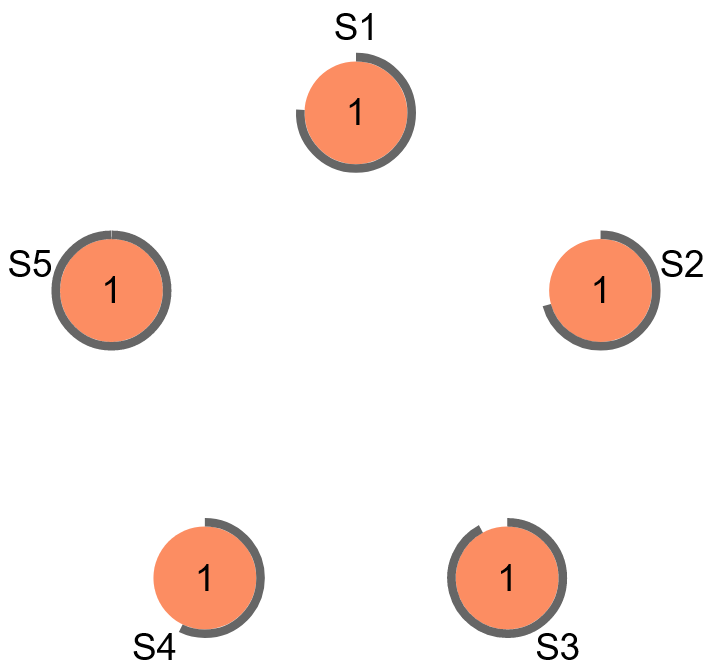
\includegraphics[width=0.45 \linewidth]{img/state_1.png}
        \label{fig:state_1}
    }
    \hfill
    \subfloat[]{
        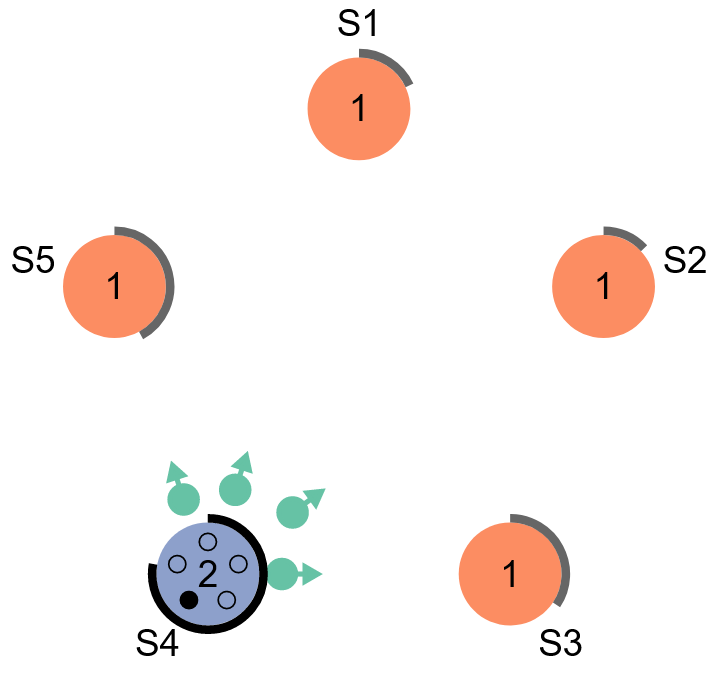
\includegraphics[width=0.45 \linewidth]{img/state_2.png}
        \label{fig:state_2}

    }
    \caption{Kai tarp mazgų nėra lyderio, mazgas, kurio rinkimų laikas yra ankščiausiai (\textit{S4}), pirmas inicijuoja naujus rinkimus ir tampa kandidatu.}
\end{figure}

Kai ateina rinkimų laikas, mazgas tampa kandidatu ir yra pradedami nauji lyderio rinkimai. \textit{S4} padidina savo terminą, balsuoja šiame rinkimų termine už save ir išsiunčia kitiems mazgams (\textit{S1}, \textit{S2}, \textit{S3}, \textit{S5}) prašymą balsuoti už jį. Prie šios užklausos yra pridedama informacija apie \textit{S4} žurnalą, kad mazgai galėtų nuspręsti, ar kandidatas \textit{S4} yra tinkamas lyderis ir ar jam reikia atiduoti savo balsą. Mazgui \textit{S4} reikia surinkti tris iš penkių balsų, taip užtikrinus daugumos pritarimą. \ref{fig:state_2} pav. surinkti balsai pavaizduoti kaip užtušuoti juodi apskritimai viduje mazgo.

\begin{figure}[H]
\centering
    \subfloat[]{
        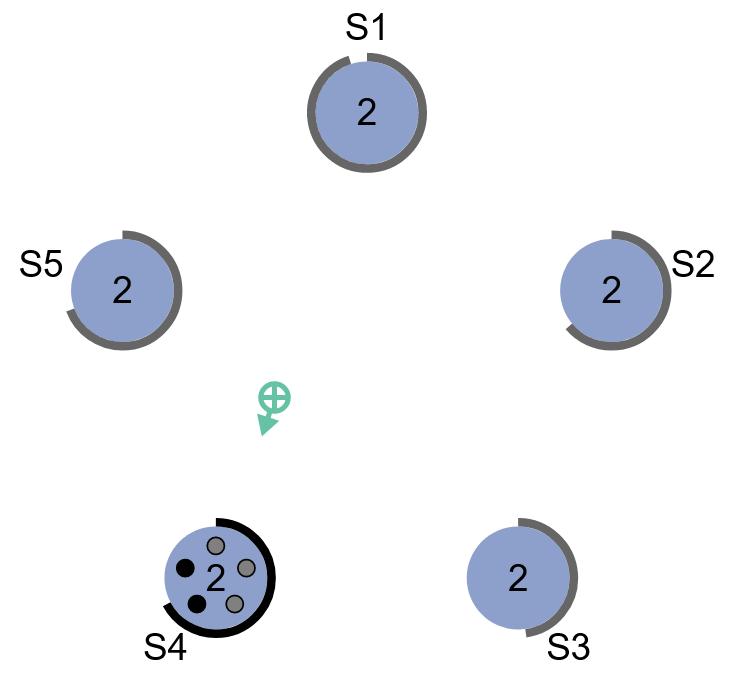
\includegraphics[width=0.45 \linewidth]{img/state_3.png}
        \label{fig:state_3}
    }
    \hfill
    \subfloat[]{
        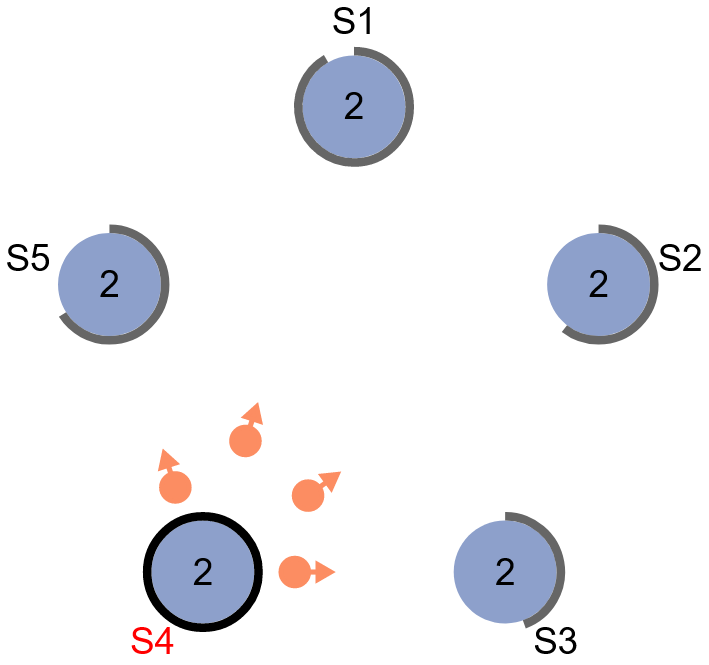
\includegraphics[width=0.45 \linewidth]{img/state_4.png}
        \label{fig:state_4}
    }
    
    \caption{Gavus daugumą balsų, mazgas--kandidatas (\textit{S4}) tampa lyderiu.}

\end{figure}

\ref{fig:state_3} pav. \textit{S4} jau surinko du balsus -- vieną iš savęs, kitą iš kito mazgo. Gavus trečią, paskutinį reikalingą, balsą, \textit{S4} tampa lyderiu ir išsiunčia kitiems mazgams savo širdies plakimo užklausą (žr. \ref{fig:state_4} pav.). Gavus lyderio užklausą, kiti mazgai iš naujo nustato rinkimų laiką. 

\subsection{Raft įrašų perdavimas}

Išrinktas lyderis aptarnauja klientus; jei užklausas iš klientų gauna mazgas kuris nėra lyderis, jis persiunčia užklausą lyderiui. Iš kliento lyderis gauna užklausą su nusakytu veiksmu, kurį reikia atlikti išskirstytai sistemai kaip būsenų mašinai. Gautą žinutę lyderis prideda į savo žurnalą kaip naują įrašą, tada asinchroniškai išsiunčia įrašo pridėjimo užklausas sekėjams. Kai dauguma sekėjų sėkmingai prideda įrašą į savo žurnalą, įrašas yra pažymimas kaip užfiksuotas (angl. \textit{committed}), įvykdomas atitinkamas įrašo veiksmas mazgų būsenų mašinoms ir lyderis grąžina rezultatą klientui~\cite{ongaro_consensus}. 

Jei dalis mazgų nustojo veikti ar lėtai grąžina atsakymus, lyderis pakartotinai siunčia įrašų pridėjimo užklausas tiems sekėjams, kurie dar nepatvirtino įrašo gavimo. Galiausiai visi mazgai turės visus žurnalo įrašus. Šis pakartotinio informacijos siuntimo procesas gali vykti net jau lyderiui išsiuntus atsakymą klientui. Tai užtikrina sistemos gyvybingumą kai mažesnioji dalis mazgų yra nepasiekiami~\cite{ongaro_consensus}.

\subsection{Raft mazgų tinklo trūkių neigiamų pasekmių sumažinimas}

Pagal klasikinį Raft, nutikus mazgų tinklo trūkiui, tai yra kai dalis mazgų tampa nepasiekiama kitai daliai mazgų, įvyksta papildomas lyderio išrinkimas -- atsijungusi dalis mazgų nepasiekia buvusio lyderio ir, praėjus rinkimų laikui, pradeda naują terminą (padidina kadencijos numerį). Kaip pasekmė, susijungus šioms mazgų dalims atgal į vieną tinklą, didesnė dalis mazgų gauna užklausas iš mažesnės dalies mazgų, kuriuose nurodytas terminas yra didesnis. Tada didesnės dalies mazgų lyderis atsistatydina, ir prasideda nauji rinkimai~\cite{ongaro_consensus}. Per trūkio laiką nauji įrašai galėtų būti užfiksuoti tik didesnėje dalyje mazgų, nes mažesnėje nebūtų galima gauti daugumos patvirtinimo. Jeigu per trūkio laiką buvo užfiksuota naujų įrašų, tai reikštų, kad lyderiu galėtų būti išrinktas tik vienas iš tos didesnės mazgų grupės narių. Vienas iš šitų mazgų yra trūkio pabaigoje esantis lyderis. Taigi, yra vykdomi papildomi rinkimai, nors galėtų būti paliktas esamas lyderis.

Šioms klasterių apjungimo pasekmėms pašalinti Raft autoriai siūlo padaryti algoritmo praplėtimą: įvesti dar vieną mazgų būseną tarp ,,sekėjo'' ir ,,kandidato'' būsenų -- ,,pirminis balsavimas'' (angl. \textit{pre-vote}). Šioje būsenoje kandidatas pradeda lyderio rinkimus tik sužinojęs, kad dauguma mazgų balsuotų už jį kaip lyderį. Mazgo terminas šioje būsenoje nėra padidinamas. Šis sprendimas išsprendžia trikdžius daliai mazgų prisijungiant atgal į didesnį mazgų klasterį, nes mažesnėje dalyje mazgų niekada nebus padidintas kadencijos numeris~\cite{ongaro_consensus}.

\section{Raft algoritmo įgyvendinimas Ra}

Šioje dalyje yra apžvelgiamas Raft algoritmo įgyvendinimas Ra. Ra yra atviro kodo Raft algoritmo biblioteka, naudojama atviro kodo žinučių brokeryje RabbitMQ\footnote{https://www.rabbitmq.com/}. Ra biblioteka yra naudojama RabbitMQ komandos išskirstytoms eilėms įgyvendinti, tačiau yra laisvai prieinama ir gali būti naudojama kaip bendra Raft biblioteka. Ra yra įgyvendinta Erlang\footnote{https://www.erlang.org/} kalba.

Nors didžioji dalis Raft algoritmo savybių yra įgyvendintos pagal Raft specifikaciją, dėl Erlang kalbos ypatybių ir konkrečių naudojimo scenarijų Ra skiriasi nuo specifikacijos, pavyzdžiui, žurnalo perdavimo ir gedimų aptikimo algoritmais~\cite{rabbitmqra}.

Pirmoje dalyje apžvelgsime Erlang kalbos ypatybes, kurios nulėmė Ra pasirinktus įgyvendinimo sprendimus. Antroje dalyje apžvelgsime Raft praplėtimus, padarytus Ra bibliotekoje. Trečioje dalyje yra detaliau išnagrinėjamas Ra naudojamas klaidų aptikimo mechanizmas ir palyginamas su Raft pasiūlytų širdies plakimo mechanizmu naudojant \texttt{AppendEntries} užklausas.

\subsection{Išskirstytas programavimas Erlang}

Erlang yra funkcinė programavimo kalba leidžianti kurti išskirstytas, atsparias gedimams, ir didelio prieinamumo reikalaujančias sistemas. Pavadinimas ,,Erlang'' gali būti naudojamas kaip sinonimas ,,Erlang/OTP'', kur OTP (angl. \textit{Open Telecom Platform}, šiame darbe naudojame anglišką santrumpą) yra karkasas skirtas supaprastinti skirtingų sistemų bendrų bruožų įgyvendinimą; OTP yra prieinamas kartu su Erlang kalba ir yra standartinės bibliotekos, kaip kalbos C++ bibliotekos \texttt{std}, atitikmuo~\cite{erlang_introduction}. Šiame darbe autoriai pavadinimą ,,Erlang'' naudojame tik Erlang programavimo kalbai vadinti.

Išskirstytas programavimas Erlang yra pagrįstas aktorių modeliu~\cite{farrugia_towards_nodate, agha_actors_1985}. Pagrindinis Erlang vykdymo vienetas yra mazgas (angl. \textit{node}) -- tai yra Erlang virtualios mašinos vienetas (išskirstytos sistemos vienetus taip pat vadinsime mazgais). Erlang mazgas gali turėti tūkstančius jame vykdomų procesų (angl. \textit{process}), o procesai komunikuoja vienas su kitu žinučių pagalba (angl. \textit{message}). Vienam iš procesų nustojus veikti, kiti procesai neįtakojami ir tęsia savo darbą. Nenumatytoms klaidoms suvaldyti procesai gali būti prižiūrimi prižiūrėtojo (angl. \textit{supervisor}), kuris gautų pranešimą nenumatytai klaidai įvykus ir prižiūrimam procesui nustojus veikti~\cite{erlang_distributed}.

Vienam iš mazgų sudarant ryšį su kitu mazgu (pavyzdžiui, panaudojus \texttt{net\_kernel:connect/1}), yra apsikeičiama žinomais mazgais ir taip sudaromas vienas mazgų tinklas. Erlang mazgų sistema yra labai lanksti ir leidžia vienam iš mazgų deleguoti kitam mazgui laisvai pasirinktą funkciją vykdymui (angl. \textit{arbitrary code execution}). \texttt{net\_kernel} modulio pagalba vienas iš mazgų gali prenumeruoti mazgų statusų pakeitimų žinučių gavimą. Tokiu atveju, pasikeitus žinomo mazgo statusui, mazgas gaus pranešimą su nauju atitinkamo mazgo statusu~\cite{erlang_distributed, hebert_learn_2013}.

Erlang mazgai palaiko ryšį tarp vienas kito ,,širdies plakimo'' (angl. \emph{heartbeat}) mechanizmo pagalba. \texttt{ticktime} yra širdies plakimo užklausos siuntimo intervalas padaugintas iš keturių ir žymi laiką, po kurio mazgas bus laikomas nepasiekiamu. Kai vienas iš mazgų negauna iš kito mazgo jo gyvavimo patvirtinančio pranešimo per \texttt{ticktime} sekundžių, tas stebimas mazgas laikomas nepasiekiamu~\cite{hebert_learn_2013}.

\subsection{Ra įgyvendinti Raft algoritmo praplėtimai}

Dėl Erlang kalbos ypatybių, konkretaus naudojimo scenarijaus ir siekio optimizuoti Raft algoritmo veikimo laiką ir naudojamų duomenų kiekį, Ra išsiskiria nuo specifikacijos kelių savybių įgyvendinimu~\cite{rabbitmqra}. Šiame skyriuje yra pateikiama Ra žurnalo perdavimo algoritmo ir Ra mazgų negyvybingumo aptikimo mechanizmų apžvalgos. 

\subsubsection{Ra žurnalo perdavimo algoritmas}

Ra nenaudoja žurnalo įrašų perdavimo užklausų mazgų gyvybingumui užtikrinti kai visų mazgų žurnalai yra sinchronizuoti. Kai vienas iš mazgų yra pasenęs, tai yra, to mazgo paskutinis sinchronizuotas įrašas yra ankstesnis negu paskutinis įrašas, siųstas lyderio tam mazgui, \texttt{AppendEntries} užklausa yra daroma, bet rečiau, negu pasiūlyta Raft specifikacijoje. Jei skirtumas tarp paskutinio sinchronizuoto įrašo ir paskutinio siųsto įrašo yra labai didelis, mazgo apkrovai sumažinti užklausos nėra siunčiamos~\cite{rabbitmqra}. Žurnalų įrašų perdavimas yra vykdomas asinchroniškai, o atsakymai yra grupuojami~\cite{rabbitmqra}.

Šiuo praplėtimo atveju Ra autoriai išnaudojo Erlang kalbos galimybes, nes Erlang leidžia palaikyti ryšį tarp mazgų išreikštinai nesiunčiant papildomų užklausų. Nesiunčiant papildomų užklausų taip pat yra atlaisvinamas ryšio kanalas, leidžiant pačiam Erlang efektyviai palaikyti ryšius ir daryti širdies plakimo užklausas~\cite{rabbitmqra}. Šiame darbe šis praplėtimas detaliau nenagrinėjamas.

\subsubsection{Ra gedimų aptikimo algoritmas}

Ra nenaudoja Raft aprašyto gedimo aptikimo algoritmo. Ra naudoja gimtąją Erlang mazgų stebėjimo infrastruktūrą stebėti ar mazgai nenustojo veikti ir kartu pasitelkia Aten\footnote{https://github.com/rabbitmq/aten} biblioteka mazgų susisiekimo klaidoms aptikti~\cite{rabbitmqra}. Aten yra adaptyvus kaupiamasis gedimų aptikimo algoritmas (angl. \textit{accrual failure detection algorithm}), kuris atsižvelgia į širdies plakimų istoriją ir pagal tai nusprendžia, ar yra didelė tikimybė nesulaukti sekančio gyvumo patvirtinimo. Tai yra naudinga siekiant sumažinti klaidingai teigiamų gedimo rezultatų skaičių didelio tinklo apkrovos metu~\cite{satzger2007_new_accrual_failure}.  

Gimtieji Erlang monitoriai leidžia greitai aptikti mazgų neveikimą procesui sustojus veikti nenumatytos klaidos metimo atveju (angl. \textit{crash}). Stebėtojui yra išsiunčiama \texttt{'DOWN'} žinutė~\cite{ericsson_erlang_processes_2016}. Erlang monitoriai užtikrina, kad sekėjai greitai sužino apie lyderio neveikimą, ir taip iš dalies pakeičia Raft širdies plakimo mechanizmą~\cite{rabbitmqra}. Aten biblioteka leidžia aptikti tinklo paskirstymo problemas, kaip mazgų nepasiekiamumą per tinklą. Kai Aten įtaria, kad vienas iš mazgų yra nepasiekiamas, yra išsiunčiama \texttt{nodedown} žinutė mazgo stebėtojui. Atitinkamai, jei mazgas ,,atsigauna'' ir atrodo vėl veikiantis, yra išsiunčiama \texttt{nodeup} žinutė~\cite{rabbitmq_aten_2020}. Kartu Erlang monitoriai ir Aten biblioteka, anot Ra autorių, užtikrina mazgų gyvumą ir pakeičia Raft aprašytą širdies plakimo mechanizmą~\cite{rabbitmqra}. 

Ra bibliotekoje visi mazgai kurie naudoja Raft algoritmą yra įgyvendinti kaip būsenų mašinos Erlang modulio \texttt{gen\_statem} \footnote{http://erlang.org/doc/man/gen\_statem.html} pagalba. 
Pirmiausia būsenų mašina prenumeruoja gauti pranešimus apie mazgų statusų pokyčius naudojant \texttt{net\_kernel:monitor\_nodes/1}\footnote{http://erlang.org/doc/man/net\_kernel.html\#monitor\_nodes-1} funkciją. Kai vienas iš mazgų tampa neprieinamas, procesas gauna \texttt{'DOWN'} pranešimą ir įvykdo atitinkamą Raft algoritmo logiką. Neprieinamumo tikrinimo laiką \texttt{ticktime} naudotojas nustato pagal savo poreikį konfigūracinio parametro pagalba~\cite{rabbitmqra}.

Taigi, Ra naudoja Erlang monitorius kiekvieno iš mazgų būsenoms stebėti. Tai leidžia palengvinti įgyvendinimo kaštus, nes didžioji dalis širdies plakimo mechanizmo algoritmo yra paimama iš Erlang OTP bibliotekos. Mazgui netikėtai nustojus veikti, klaida bus aptikta iškarto ir stebėtojui bus išsiųsta \texttt{'DOWN'} žinutė, o mazgui lėtai atsakant ar ryšiui nutrūkus, nepasiekiamumą padės nustatyti širdies plakimo mechanizmas paremtas adaptyviu kaupiamuoju gedimų aptikimo algoritmu.

\section{Ra gedimų aptikimo algoritmo formali specifikacija}

Ra bibliotekos Raft algoritmo įgyvendinimo korektiškumo užtikrinimo sudėtingumui sumažinti, šio darbo metu buvo praplėsta Raft algoritmo formalios specifikacijos dalis susijusi su gedimų aptikimo algoritmu. Taip pat sukurta ir Ra bibliotekos gedimų aptikimo algoritmo formali specifikacija. Šioje dalyje yra pateikiamos šių dviejų formalių gedimų aptikimo algoritmo specifikacijų (toliau -- specifikacijų), parašytų TLA$^+$ kalba, aprašymai. Specifikacijos yra pateikiamos kaip darbo priedai. Specifikacijų išeities tekstai yra viešai pasiekiami adresu: \url{https://github.com/EdvardasDlugauskas/Coursework-2020}. Šių dviejų algoritmų vienodos elgsenos įrodymas nėra pateikiamas ir lieka būsimiems darbams. 

Pagrindinis Raft ir Ra gedimo aptikimo algoritmų formalių specifikacijų kūrimo tikslas yra formaliai aprašyti Ra mazgų gedimo aptikimo mechanizmą, kas vėliau padėtų įrodyti Ra įgyvendinimo Raft specifikacijos atitikimą ir Raft savybių išlaikymą. Raft autoriai pateikė Raft formaliosios specifikacijos pradinį kodą, tačiau jame gedimų aptikimo algoritmas yra suabstrahuotas kaip vienas žingsnis -- sekėjo rinkimo laiko pasibaigimas ir perėjimas į sekančią būseną, pradiniam kode tai nurodo funkcija \texttt{Timeout}~\cite{ongaro_consensus}. Detalesniam Raft ir Ra gedimo aptikimo mechanizmų palyginimui šio darbo autoriai, remiantis Raft specifikacija, sukūrė detalesnę Raft gedimo aptikimo algoritmo specifikaciją, kuri yra pateikta \ref{sec:appendix_raft_tla_spec}~priede. Ra gedimų aptikimo algoritmo specifikacija yra sukurta panašiu detalumo lygiu siekiant palengvinti šių dviejų specifikacijų palyginimą. Pilna Ra gedimų aptikimo algoritmo specifikacija yra pateikta \ref{sec:appendix_ra_tla_spec}~priede.

Šių specifikacijų rašymo metu buvo laikomasi tokių pat prielaidų kaip Raft formalioje specifikacijoje (žr. \ref{section:raft_intro} skyrių).

Pagal Raft, pasikeitus lyderiui, naujojo lyderio terminas bus didesnis, kas privers sekėją padidinti ir savo vidinį terminą, pagal kurį galima ignoruoti senesnių lyderių pavėlavusias užklausas (nes juose nurodytas terminas bus senesnis). Tai leidžia supaprastinti specifikaciją iki vieno lyderio--sekėjo ryšio tyrimo. Specifikacijų sritis ir yra dviejų mazgų -- lyderio ir sekėjo -- ryšio palaikymas ir sekėjo lyderio gedimų aptikimas. Šis lyderio--sekėjo ryšys yra nepalaikomas kai sekėjas nustato, kad lyderis nustojo veikti arba nėra pasiekiamas. Dėl to papildomai apribojame specifikacijų aprašytą sritį:

\begin{itemize}
\item Modeliuojamas tik vienas lyderio--sekėjo ryšys.
\item Lyderiui nustojus veikti ir sekėjui tai nustačius, sekėjas pereiną į sekančią būseną (,,pirminis balsavimas'' arba ,,kandidatas'') ir tolimesnis elgesys nėra aprašomas specifikacijose.
\item Pagal Raft specifikaciją, \texttt{AppendEntries} užklausa be žurnalo įrašų sekėjo būsenoje įtakoja tik \texttt{commitIndex} reikšmę~\cite{ongaro_consensus}. Todėl kitos perduodamos reikšmės nėra įtrauktos į specifikacijas. 
\end{itemize}

Formali Raft gedimo aptikimo mechanizmo specifikacija, kuri yra pateikta priede \ref{sec:appendix_raft_tla_spec}, aprašo lyderio ir vieno iš jo sekėjų ryšį, kai sekėjas gauna iš lyderio \texttt{AppendEntries} užklausas. Specifikacija apibrėžia visas galimas šio ryšio būsenas. Yra apibrėžiama pradinė būsena (\texttt{Init}), kurioje lyderis yra veikiantis bet dar neišsiuntė nė vienos užklausos, ir apibrėžiami visi galimi perėjimai iš vienos būsenos į kitą (\texttt{Next}). Tokių perėjimų yra keletas: lyderis išsiunčia žinutę; lyderis padidina savo paskutinio fiksuoto įrašo indeksą; tinklas pameta (ištrina) žinutę; sekėjas gauna žinutę ir atnaujina savo \texttt{commitIndex} reikšmę; lyderis nustoja veikti, po ko negalės atlikti jokių veiksmų; sekėjas nustato kad lyderis nepasiekiamas. 

\begin{adjustwidth}{2cm}{}

\begin{tla}
Next == \/ SendMessage
        \/ IncrementIndex
        \/ DropMessage
        \/ ReceiveMessage
        \/ CrashLeader
        \/ Timeout
\end{tla}
\begin{tlatex}
\@pvspace{8.0pt}%
\@x{ Next \.{\defeq} \.{\lor} SendMessage}%
\@x{\@s{46.5} \.{\lor} IncrementIndex}%
\@x{\@s{46.5} \.{\lor} DropMessage}%
\@x{\@s{46.5} \.{\lor} ReceiveMessage}%
\@x{\@s{46.5} \.{\lor} CrashLeader}%
\@x{\@s{46.5} \.{\lor} Timeout}%
\@pvspace{8.0pt}%
\end{tlatex}

\end{adjustwidth}


Prie kiekvieno perėjimo aprašytos sąlygos, kurias tenkinant šis perėjimas gali įvykti. Pavyzdžiui, lyderis gali siųsti užklausas tik jei jis yra veikiantis.


\begin{adjustwidth}{2cm}{}

\begin{tla}
SendMessage == 
        /\ leaderState = "ALIVE"
        /\ messages' = Append(messages, leaderIndex)
        /\ UNCHANGED <<leaderState, nodeIndexes, isTimeout>>
\end{tla}
\begin{tlatex}
\@pvspace{8.0pt}%
\@x{ SendMessage \.{\defeq}}%
\@x{\@s{32.8} \.{\land} leaderState \.{=}\@w{ALIVE}}%
 \@x{\@s{32.8} \.{\land} messages \.{'} \.{=} Append ( messages ,\,
 leaderIndex )}%
 \@x{\@s{32.8} \.{\land} {\UNCHANGED} {\langle} leaderState ,\, nodeIndexes
 ,\, isTimeout {\rangle}}%
\@pvspace{8.0pt}%
\end{tlatex}

\end{adjustwidth}


Formali Ra bibliotekos gedimo aptikimo mechanizmo specifikacija yra pateikta priede \ref{sec:appendix_ra_tla_spec} ir aprašo tą patį lyderio--sekėjo ryšį. Ra atveju širdies plakimo žinutės neneša papildomos informacijos kaip \texttt{commitIndex}, o nustojus veikti lyderiui yra išsiunčiama \texttt{nodedown} žinutė, kurią gavus sekėjas gali nelaukti kol pasibaigs rinkimų laikas. Taigi, galimi perėjimai iš vienos būsenos į kitą šiuo atveju yra: lyderis išsiunčia širdies plakimo žinutę; sekėjas gauna širdies plakimo žinutę; tinklas pameta (ištrina) širdies plakimo žinutę; lyderis nustoja veikti, yra išsiunčiama \texttt{nodedown} žinutė; sekėjas gauna \texttt{nodedown} žinutę ir iš karto pasižymi, kad lyderis yra nepasiekiamas; tinklas pameta (ištrina) \texttt{nodedown} žinutę; sekėjas nustato kad lyderis nepasiekiamas. Analogiškai su Raft specifikacija, prie kiekvieno perėjimo parašytos jam reikalingos sąlygos.

\begin{adjustwidth}{2cm}{}

\begin{tla}
Next == \/ DropHeartbeat
        \/ SendHeartbeat
        \/ ReceiveHeartbeat
        \/ DropNodedown
        \/ ReceiveNodedown
        \/ CrashLeader
        \/ Timeout
\end{tla}
\begin{tlatex}
\@pvspace{8.0pt}%
\@x{ Next \.{\defeq} \.{\lor} DropHeartbeat}%
\@x{\@s{47} \.{\lor} SendHeartbeat}%
\@x{\@s{47} \.{\lor} ReceiveHeartbeat}%
\@x{\@s{47} \.{\lor} DropNodedown}%
\@x{\@s{47} \.{\lor} ReceiveNodedown}%
\@x{\@s{47} \.{\lor} CrashLeader}%
\@x{\@s{47} \.{\lor} Timeout}%
\@pvspace{8.0pt}%
\end{tlatex}


\end{adjustwidth}

Raft gedimų aptikimo specifikacijos korektiškumui patikrinti buvo panaudotas invariantas \texttt{TypeOK}, užtikrinantis teisingus specifikacijoje naudojamų kintamųjų rėžius. Taip pat buvo panaudota savybė \texttt{LeaderFailureDetected} -- jei lyderis yra neveikiantis, kažkurioje sekančioje būsenoje bus aptiktas lyderio nepasiekiamumas.

\begin{adjustwidth}{2cm}{}

\begin{tla}
TypeOK == /\ leaderState \in {"ALIVE", "CRASHED"}
          /\ messages \in Seq(Nat)
          /\ leaderIndex \in Nat
          /\ followerIndex \in Nat      
          /\ isTimeout \in BOOLEAN

LeaderFailureDetected == leaderState = "CRASHED" ~> isTimeout = TRUE
\end{tla}
\begin{tlatex}
\@pvspace{8.0pt}%

\@x{ TypeOK \.{\defeq} \.{\land} leaderState \.{\in} \{\@w{ALIVE}, \,\@w{CRASHED} \}}%
\@x{\@s{67.4} \.{\land} messages \.{\in} Seq ( Nat )}%
\@x{\@s{67.4} \.{\land} leaderIndex \.{\in} Nat}%
\@x{\@s{67.4} \.{\land} followerIndex \.{\in} Nat}%
\@x{\@s{67.4} \.{\land} isTimeout \.{\in} {\BOOLEAN}}%
\@pvspace{8.0pt}%
\@x{ LeaderFailureDetected \.{\defeq} leaderState \.{=}\@w{CRASHED} \.{\leadsto} isTimeout \.{=} {\TRUE}}%

\@pvspace{8.0pt}%
\end{tlatex}

\end{adjustwidth}

Raft gedimo aptikimo specifikacijai buvo sukurtas TLA$^+$ modelis ir apribota tikrinamų būsenų aibė: lyderio indeksas turi būti mažesnis 10, o žinučių, vienu metu esamų tinkle, skaičius -- mažesnis nei 5. Savybėms patikrinti buvo panaudotas TLC modelio būsenų tikrinimo įrankis, integruotas į TLA$^+$ Toolbox darbo aplinką. Iš viso buvo patikrinta virš 80 tūkstančių unikalių būsenų, kiekvienai iš kurių galiojo aprašytos kintamųjų rėžių ir lyderio gedimo aptikimo savybės. Ra gedimo aptikimo specifikacijai buvo sukurtos ir patikrintos atitinkamos \texttt{TypeOK} ir \texttt{LeaderFailureDetected} savybės, buvo apribota tikrinamų būsenų aibė -- širdies plakimo užklausų gali būti ne daugiau kaip 13. Visos modelio rastos būsenos (iš viso unikalių apie 100 tūkstančių) atitiko apibrėžtas savybes. 

Palyginus specifikacijas, galima teigti, kad, išskyrus \texttt{commitIndex} perdavimą sekėjui, Ra algoritmas atlieka tuos pačius veiksmus kaip Raft algoritmas, bet papildomai turi \texttt{nodedown} žinučių perdavimo mechanizmą. Mūsų nuomone, tai parodo, kad Ra įgyvendinimas atitinka Raft specifikaciją, tačiau formaliam įrodymui reikia ištirti \texttt{commitIndex} nebuvimo širdies plakimo žinutėse pasekmes ir formaliai įrodyti dviejų algoritmų ekvivalentiškumą. Tai yra paliekama ateities darbams.

\sectionnonum{Rezultatai ir išvados}

Mūsų nuomone, Raft algoritmo įgyvendinimas Ra yra gerokai palengvinamas tuo, kad gimtosios Erlang funkcijos ir bibliotekos yra skirtos būtent tokių išskirstytų sistemų būsenų stebėjimui, todėl įgyvendinimo kaštai yra dar labiau sumažinami. Visa tai gerai komponuoja su Raft autorių motyvacija~\cite{ongaro_consensus} -- padaryti išskirstytų sistemų konsensuso algoritmo įgyvendinimą kuo paprastesnį, sumažinti galimų klaidų skaičių, leisti kuo lengviau papildyti esamą funkcionalumą naujais praplėtimais. Mūsų nuomone, Ra biblioteka yra ne tik puikus techninio Raft algoritmo įgyvendinimo, bet ir Raft paprastumo ir aiškumo dvasią išlaikančios bibliotekos pavyzdys. 

Šiame darbe buvo pasiekti rezultatai:
\begin{enumerate}
\item Pateiktos formalios Raft ir Ra gedimų aptikimo algoritmų specifikacijos parašytos TLA$^+$ kalba. Išnagrinėti jų skirtumai.
\end{enumerate}

Šio darbo padarytos išvados:
\begin{enumerate}
\item Mūsų nuomone, tarp Raft ir Ra gedimo aptikimo specifikacijų yra daug panašumų, tačiau yra ir skirtumų, kurių poveikis algoritmo veikimui neakivaizdus.
\item Ra bibliotekos Raft mazgų neveikimo aptikimo specifikacijos atitikimui formaliai įrodyti reikia ištirti \texttt{commitIndex} reikšmės nebuvimo širdies plakimo žinutėse padarinius ir formaliai įrodyti jų gedimų aptikimo algoritmų Raft savybių atitikimo ekvivalentiškumą, galimai remiantis šiame darbe pateiktomis formaliomis Raft ir Ra algoritmų specifikacijomis.
\end{enumerate}

%Rezultatų ir išvadų dalyje turi būti aiškiai išdėstomi pagrindiniai darbo
%rezultatai (kažkas išanalizuota, kažkas sukurta, kažkas įdiegta) ir pateikiamos
%išvados (daromi nagrinėtų problemų sprendimo metodų palyginimai, teikiamos
%rekomendacijos, akcentuojamos naujovės).

\printbibliography[heading=bibintoc]  % Šaltinių sąraše nurodoma panaudota
% literatūra, kitokie šaltiniai. Abėcėlės tvarka išdėstomi darbe panaudotų
% (cituotų, perfrazuotų ar bent paminėtų) mokslo leidinių, kitokių publikacijų
% bibliografiniai aprašai.  Šaltinių sąrašas spausdinamas iš naujo puslapio.
% Aprašai pateikiami netransliteruoti. Šaltinių sąraše negali būti tokių
% šaltinių, kurie nebuvo paminėti tekste.

% \sectionnonum{Sąvokų apibrėžimai}
% \sectionnonum{Santrumpos}
%Sąvokų apibrėžimai ir santrumpų sąrašas sudaromas tada, kai darbo tekste
%vartojami specialūs paaiškinimo reikalaujantys terminai ir rečiau sutinkamos
%santrumpos.

\appendix  % Priedai

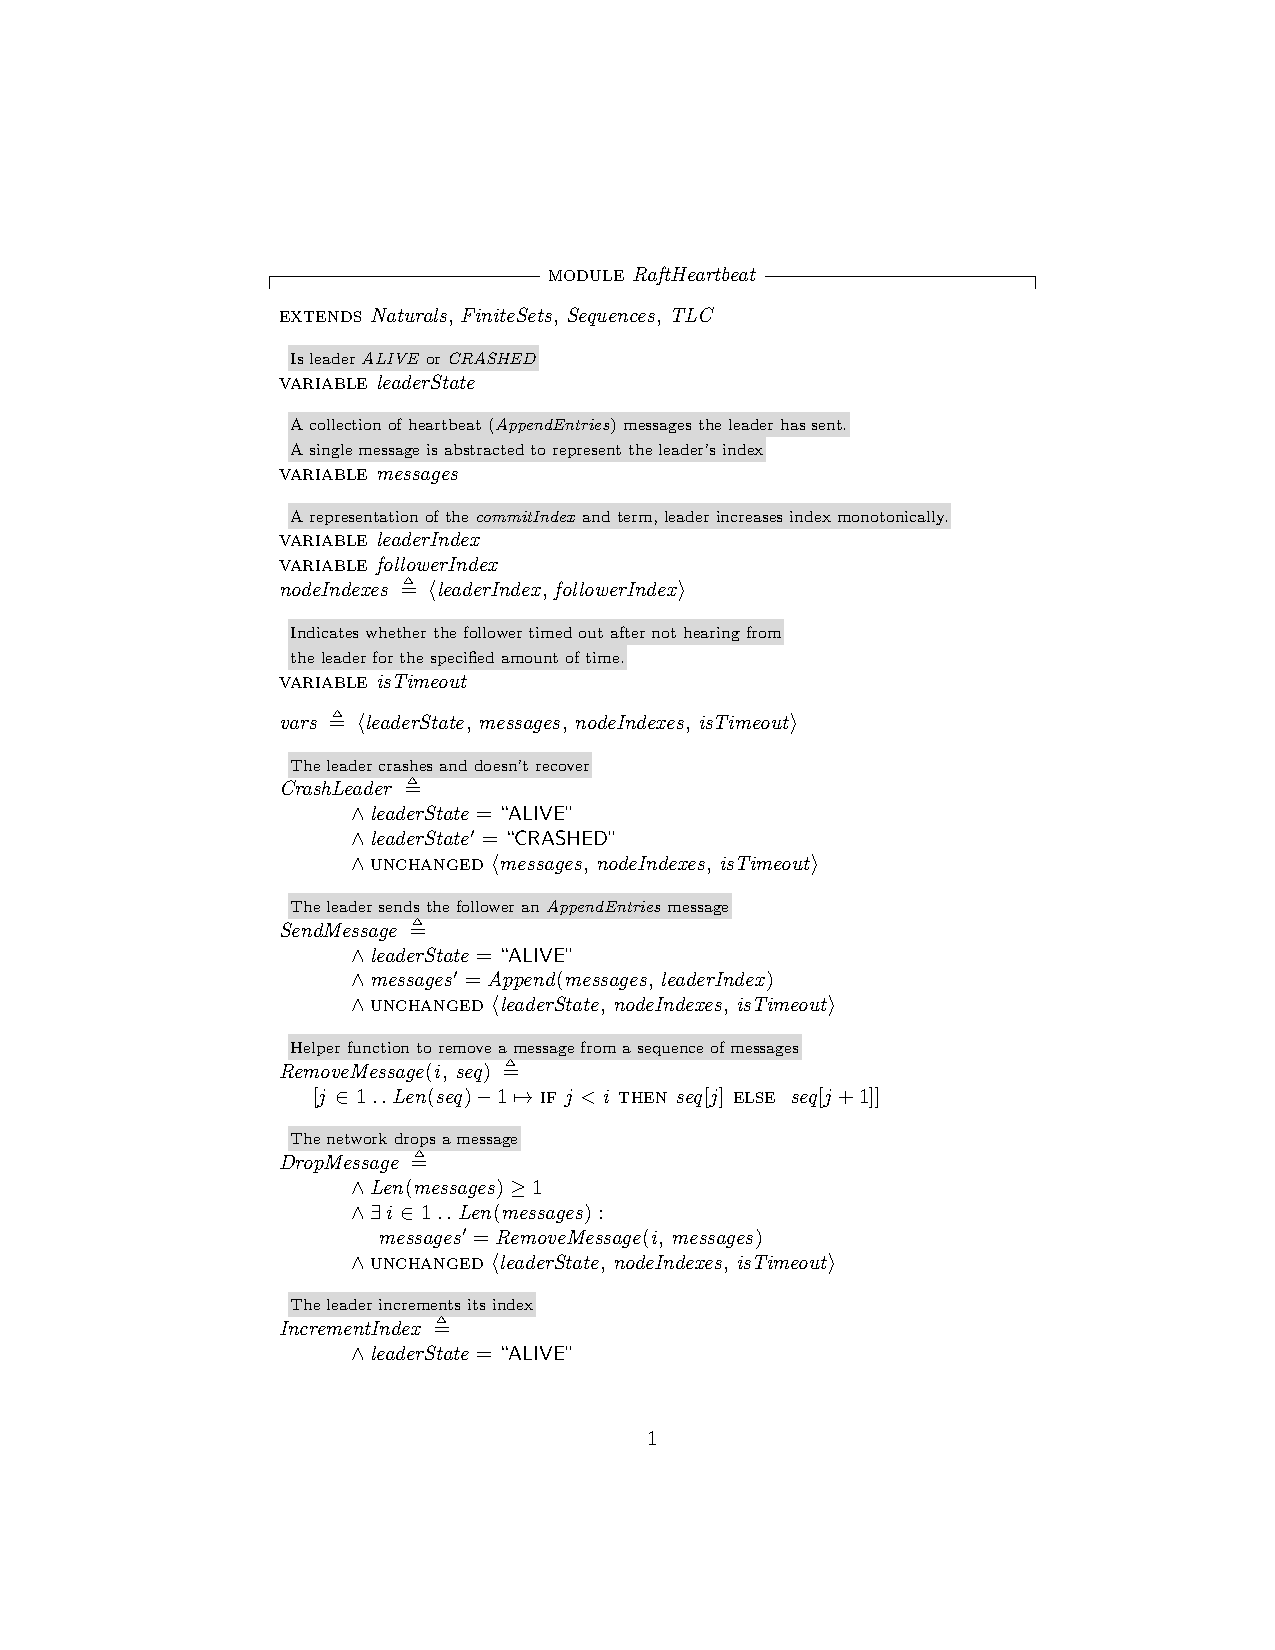
\includepdf[pages=1, pagecommand=\section{Raft algoritmo gedimo aptikimo specifikacija TLA$^+$ kalba}\label{sec:appendix_raft_tla_spec}]{spec/RaftHeartbeat.pdf}
\includepdf[pages=2-, pagecommand={}]{spec/RaftHeartbeat.pdf}

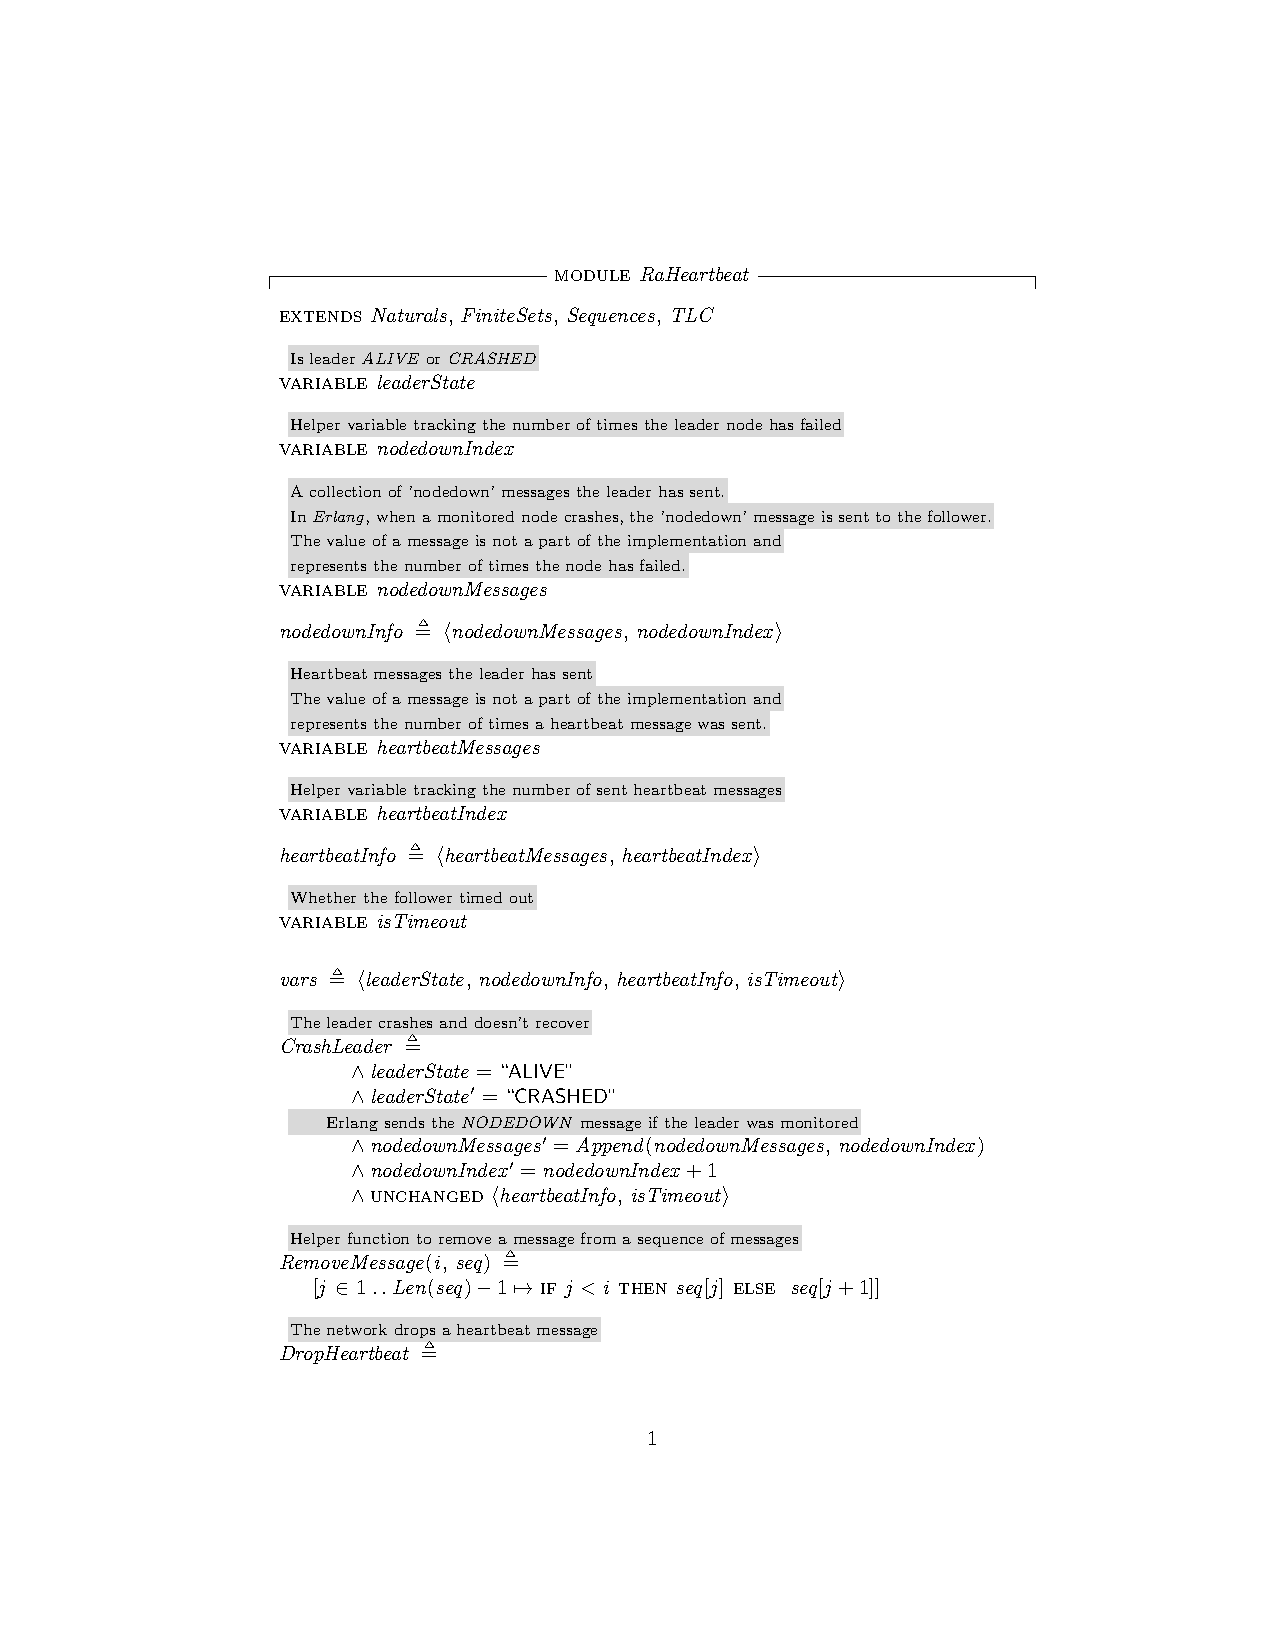
\includepdf[pages=1, pagecommand=\section{Ra bibliotekos gedimo aptikimo specifikacija TLA$^+$ kalba}\label{sec:appendix_ra_tla_spec}]{spec/RaHeartbeat.pdf}
\includepdf[pages=2-, pagecommand={}]{spec/RaHeartbeat.pdf}

% Prieduose gali būti pateikiama pagalbinė, ypač darbo autoriaus savarankiškai
% parengta, medžiaga. Savarankiški priedai gali būti pateikiami ir
% kompaktiniame diske. Priedai taip pat numeruojami ir vadinami. Darbo tekstas
% su priedais susiejamas nuorodomis.

\end{document}